\documentclass[a4paper,12pt]{article}
\usepackage[utf8]{inputenc}
\usepackage[spanish]{babel}
\usepackage{amsmath}
\usepackage{amssymb}
\usepackage{geometry}
\usepackage{graphicx}
\usepackage{graphics}
\usepackage{listings}
\usepackage{xcolor}  % for coloring
\renewcommand{\lstlistingname}{Código}
\renewcommand{\lstlistlistingname}{Índice de códigos}

\lstset{
  language=python,                   % Idioma del código
  basicstyle=\ttfamily\small,  % Fuente monoespaciada pequeña
  keywordstyle=\color{blue}\bfseries, % Palabras clave en azul y negrita
  commentstyle=\color{gray},   % Comentarios en gris
  stringstyle=\color{red},     % Cadenas en rojo
  numbers=left,                % Numerar líneas a la izquierda
  numberstyle=\tiny,           % Tamaño de los números de línea
  numbersep=5pt,               % Separación de los números
  backgroundcolor=\color{white}, % Fondo blanco
  frame=single,                % Marco alrededor del código
  breaklines=true,             % Romper líneas largas
  captionpos=b,                % Colocar el título debajo del código
  literate={á}{{\'a}}1 {é}{{\'e}}1 {í}{{\'i}}1 {ó}{{\'o}}1 {ú}{{\'u}}1 {ñ}{{\~n}}1 {Ñ}{{\~N}}1, % Soporte para caracteres especiales
  extendedchars=true,
  columns=flexible,
  inputencoding=utf8
}
\usepackage[%  
    colorlinks=true,
    pdfborder={0 0 0},
    linkcolor=red
]{hyperref}
\geometry{margin=2.5cm}

\title{Informe de Trabajo Práctico 4}
\author{Aprendizaje Profundo con aplicación a Visión Artificial \\
Laura Zúñiga Osorio}
\date{\today}

\begin{document}
\maketitle

\section{Cálculo de DKL}
En este ejercicio probamos algunas probabilidades de la Divergencia de Kullback-Leibler, definida como:
\begin{equation}
    D_{KL} (p||q) = \int p(x) \log{\frac{p(x)}{q(x)}} dx~.
\end{equation}

\paragraph{No negatividad.} Usamos el hecho de que $\log{t}\leq t-1~ \forall~ t>0$. Tomamos $t=\dfrac{q(x)}{p(x)}$ (con $p(x)>0$). Entonces
\begin{align*}
D_{KL}(p\|q)
&= \int p(x)\log\frac{p(x)}{q(x)}\,dx
= -\int p(x)\log\frac{q(x)}{p(x)}\,dx\\
&\ge -\int p(x)\!\left(\frac{q(x)}{p(x)}-1\right)\!dx
= -\int q(x)\,dx + \int p(x)\,dx = -1+1 = 0.
\end{align*}
Por tanto, $D_{KL}(p\|q)\ge 0$.


\paragraph{Deducción de la cota variacional.} 

En primer lugar, sabemos que la integral de una distribución de probabilidad es 1. Por tanto,

\begin{equation}
    \log{p(x)} = \log{p(x)}\cdot 1 = \log{p(x)}\int q(z|x)dz =  \int q(z|x)\log{p(x)} dz.
\end{equation}
La regla de Bayes nos dice que $p(x,z)=p(x)p(z|x)$, entonces $\log{p(x)} = \log{\frac{p(x,z)}{p(z|x)}}$.
Escribimos 
\begin{equation}
    \log{p(x)} = \int q(z|x) \log{p(x)} dz = \int q(z|x) \log{\frac{p(x,z)}{p(z|x)}} dz
\end{equation}
Dividiendo arriba y abajo por $q(z|x)$ dentro del logaritmo:

\begin{align}
    \log{p(x)} &= \int q(z|x) \log{\frac{p(x,z) q(z|x)}{p(z|x)q(z|x)}} dz \\
    &= \int q(z|x) \left[ \log{\frac{q(z|x)}{p(z|x)}}+\log{\frac{p(x,z)}{q(z|x)}} dz \right] \\
    &= \int q(z|x) \log{\frac{q(z|x)}{p(z|x)}}dz + \int q(z|x)\log{\frac{p(x,z)}{q(z|x)}}dz \\
    &= D_{KL}(q(\cdot|x)~||~p(\cdot|x)) + \int q(z|x)\log{\frac{p(x,z)}{q(z|x)}}dz
\end{align}

\paragraph{Obtención de error de reconstrucción + $\mathbf{\hat{D}_{KL}}$ .} Partimos del último término de la eq. (7), reescribiéndolo (por Bayes) como
\begin{align}
    B &= \int q(z|x)\log{\frac{p(z)p(x|z)}{q(z|x)}}dz \\
      &=  \left[\int q(z|x)  \log{p(x|z)} -\log{\frac{q(z|x)}{p(z)}} \right] dz \\
      &=  \left[\int q(z|x)  \log{p(x|z)}dz\right] - \left[\int q(z|x)\log{\frac{q(z|x)}{p(z)}} \right] dz \\
      &=  \left[\int q(z|x) \log{p(x|z)} dz \right] - D_{KL} (q(\cdot|x)||p(\cdot))
\end{align}

\paragraph{Cálculo para distribución Gaussiana.}
Si \(p=\mathcal{N}(\mu_p,\sigma_p^2)\) y \(q=\mathcal{N}(\mu_q,\sigma_q^2)\), entonces
\begin{align}
D_{KL}(p\|q)    &= \int p(x)\log\frac{p(x)}{q(x)}\,dx \\
&= \int p(x)\left[\log{\frac{\sigma_q}{\sigma_p}}    +\frac{(x-\mu_q)^2}{2\sigma_q^2}-\frac{(x-\mu_p)^2}{2\sigma_p^2}\right]dx \\
&= \log{\frac{\sigma_q}{\sigma_p}}    +\frac{1}{2\sigma_q^2}\mathbb{E}_p\!\left[(x-\mu_q)^2\right]    -\frac{1}{2\sigma_p^2}\mathbb{E}_p\!\left[(x-\mu_p)^2\right] \\
&= \log{\frac{\sigma_q}{\sigma_p}}    +\frac{\sigma_p^2+(\mu_p-\mu_q)^2}{2\sigma_q^2}    -\frac{1}{2} \\
&= \log{\frac{\sigma_q}{\sigma_p}} +\frac{\sigma_p^2+(\mu_p-\mu_q)^2}{2\sigma_q^2}-\frac{1}{2}.
\end{align}
\newpage
\section{Auto-encoder variacional}
En este ejercicio entrenamos y evaluamos la performance de un autoencoder variacional convolucional que aprende a generar dígitos manuscritos a partir de la base de datos MNIST.
Para ello, construimos una red del tipo encoder-decoder con la siguiente arquitectura:

\begin{figure}[!ht]
    \centering
    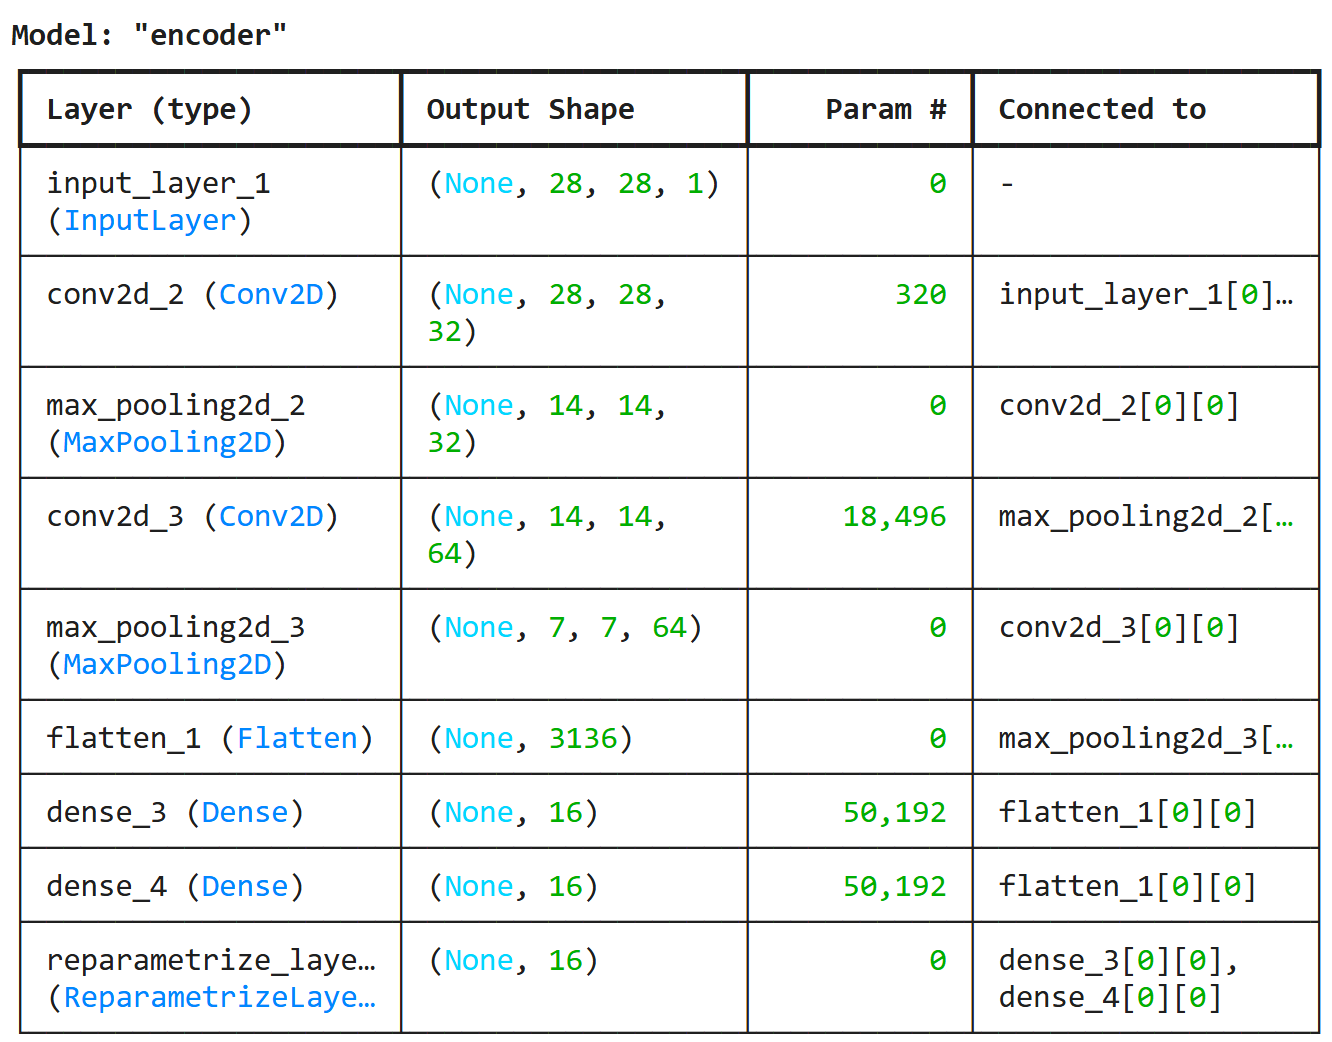
\includegraphics[width=0.7\textwidth]{encoder.png}
    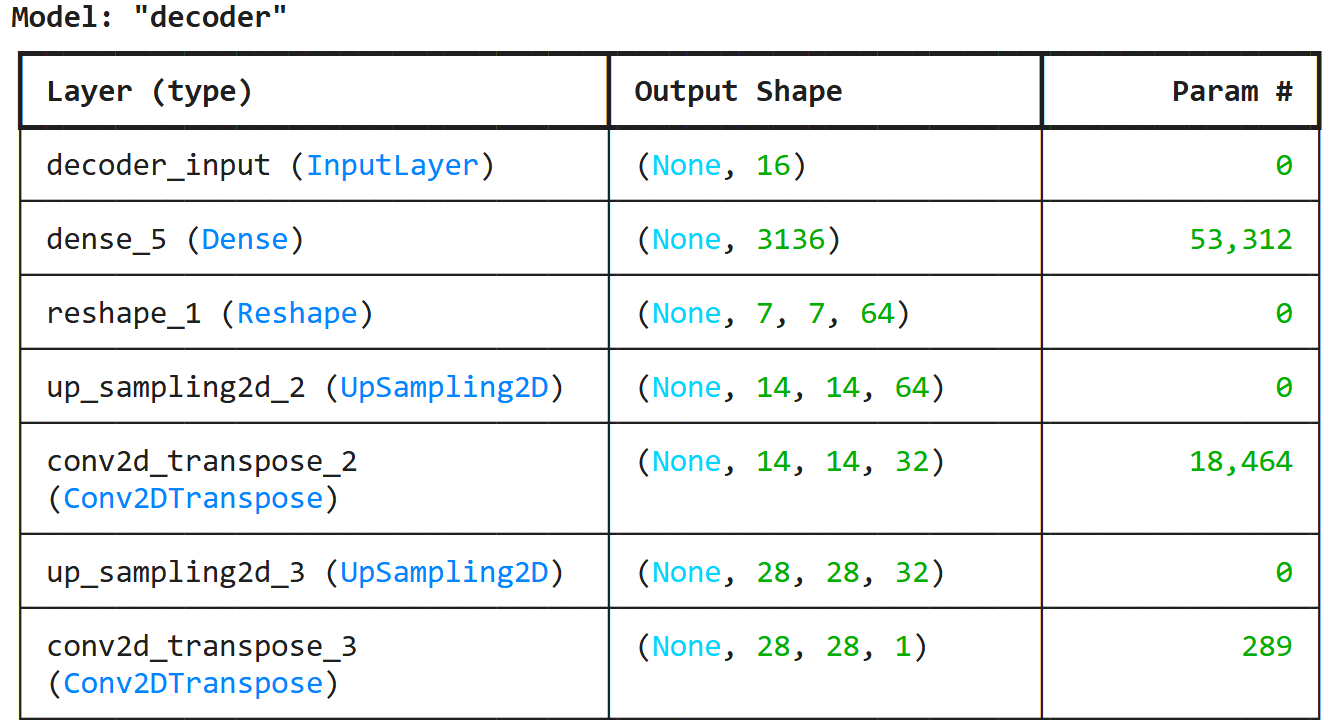
\includegraphics[width=0.7\textwidth]{decoder.png}
    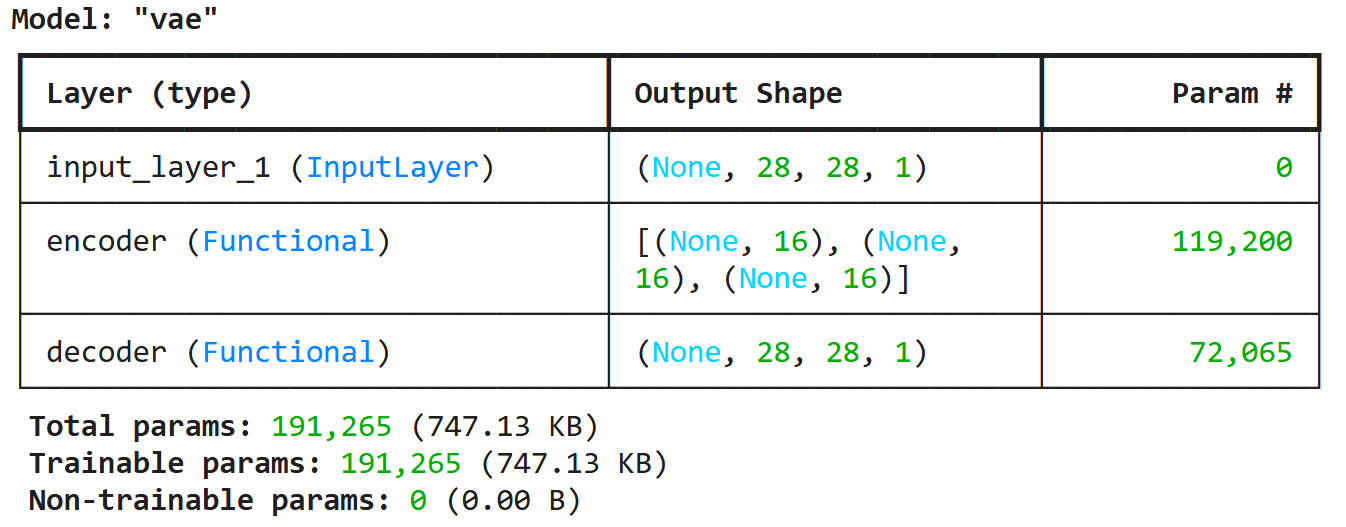
\includegraphics[width=0.7\textwidth]{vae.png}
    \caption{Arquitectura de autoencoder variacional convolucional, separando en redes distintas al encoder y el decoder.}
\end{figure}

La capa de reparametrización se encarga de muestrear puntos en el espacio latente para servir como entradas al decoder. Está definida de la forma:

\begin{lstlisting}[language=python]
class ReparametrizeLayer(keras.Layer):
def call(self, mu, logvar, training=None):
    self.mu = mu
    self.logvar = logvar
    std = tf.exp(0.5 * logvar)
    if training:
        eps = tf.random.normal(shape=tf.shape(std))
        return mu + eps * std
    else:
        return mu
\end{lstlisting}

La red se entrenó por 100 épocas usando como función de pérdida el error de reconstrucción y la Divergencia de Kullback Leibler entre las distribuciones de entrada (conjunto de entrenamiento) y de salida (predicciones).
Los dígitos generados a partir de 10 puntos sampleados del ReparametrizeLayer se muestran a continuación:

\begin{figure}[!ht]
    \centering
    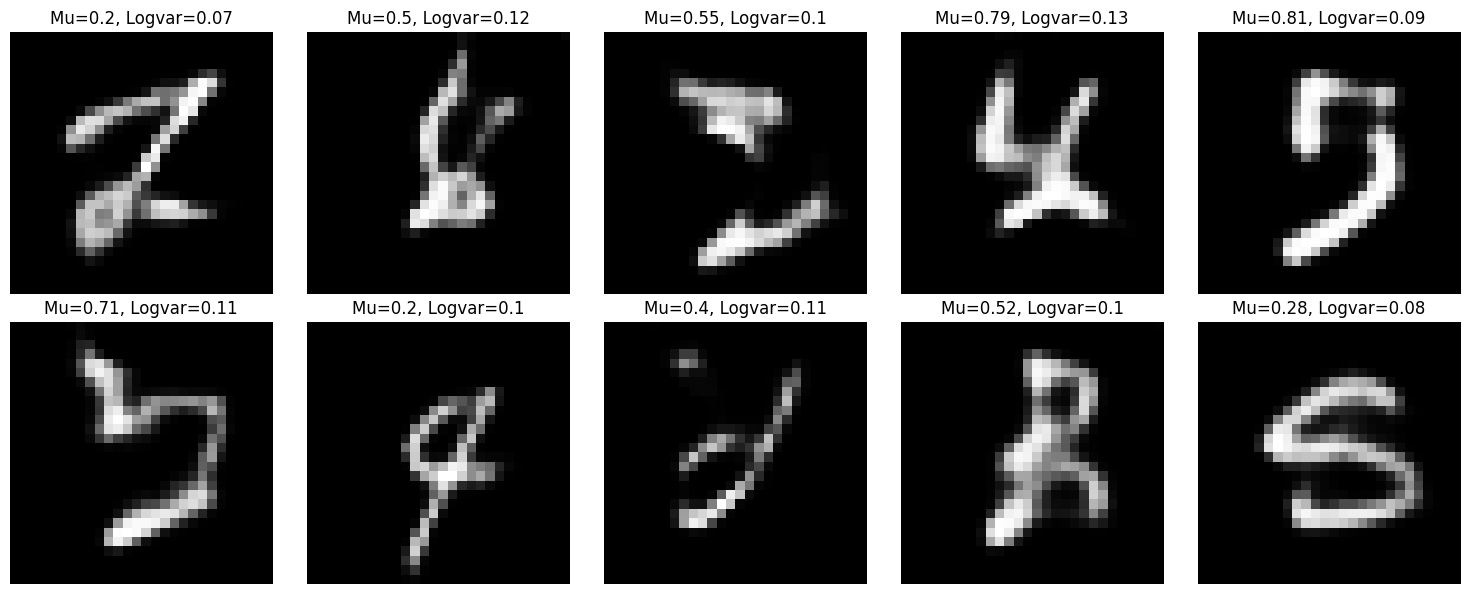
\includegraphics[width=\textwidth]{res2.png}
    \caption{Resultados de generación de dígitos a partir de muestreo de distribución normal en autoencoder variacional convolucional, entrenada con la base de datos MNIST.}
\end{figure}

\end{document}